\section{Model}

We model all $R$ regions of the cleaned time series $(t, x)$ with a single model that captures the gradual growth within each region as well as two features of between-region change of the growth rate ($\mu$), sudden changes and long-term drifts.

\subsection{Parameters}
We use the following unknown variables to describe the time series. The role of each value will become more clear in the next subsection.
\begin{itemize}
	\item $x_0 = \{x_{r,0}\;:\;r=1,2,\ldots R\} \in \mathds{R}^R$ represents the starting log-OD value at the beginning of each region.
	\item $\mu_1 = \{\mu_{r,1}\;:\;r=1,2,\ldots R\} \in \mathds{R}^R$  represents the growth rate at the beginning of each region.
	\item $\mu_2 = \{\mu_{r,2}\;:\;r=1,2,\ldots R\} \in \mathds{R}^R$  represents the growth rate at the end of each region.
	\item $\sigma_x \in \mathds{R}$ is the strength of measurement noise of log-OD.
	\item $\mu_0$ is $\mu$ at the beginning of the experiment.
	\item $\nu_0$ is the \emph{rate of change} of $\mu$ at the beginning of the experiment
	\item $D$ is the diffusion coefficient of the velocity of the long term drift of $\mu$.
	\item $\tau$ is the time scale of the short-term fluctuations of $\mu$.
	\item $\sigma_y$ is the magnitude of the short-term fluctuations of $\mu$.
\end{itemize}


\subsection{Individual regions}
We assume that for given $x_0, \mu_1, \mu_2$ values, the log-OD values in different regions become independent. This allows us to write the generating distribution of log-OD as 
\be
	P(x\;|\;x_0, \mu_1, \mu_2, \sigma_x) = \prod_{r=1}^R P(x^{(r)}\;|\; x_{r,0}, \mu_{r,1}, \mu_{r,2}, \sigma_x)\quad ,
\ee
where $x^{(r)}$ and $t^{(r)}$ are the set of log-OD and time points belonging to region $r$.

Furthermore, within each region $r$, we assume that $\mu$ changes deterministically and linearly between $\mu_{r,1}$ (at $t_{s(r)}$) and $\mu_{r,2}$ (at $t_{e(r)}$), i.e.
\be
	\mu(t) = 
	\mu_{r,1} \frac{t_{e(r)} - t}{t_{e(r)} - t_{s(r)}} + 
	\mu_{r,2} \frac{t - t_{s(r)}}{t_{e(r)} - t_{s(r)}}\quad,\quad\text{if}\quad t_{s(r)} \leq t \leq t_{e(r)}\quad.
\ee
This leads to a quadratic time dependence for the ``noiseless'' log-OD,
\ba
	x_r^\text{noiseless}(t) 
	&=& 
	x_{r,0} + \intop_{t_{s(r)}}^{t} \d{t'} \mu(t') = 
	x_{r,0} + f_r(t)\,\mu_{r,1} + g_r(t)\,\mu_{r,2}\quad ,\text{ where }
	\\
	f_r(t) &=& \frac{t_{e(r)}(t - t_{s(r)}) - \frac{1}{2} (t^2 - t_{s(r)}^2)}{t_{e(r)} - t_{s(r)}}
	\\
	g_r(t) &=& \frac{\frac{1}{2}(t^2 - t_{s(r)}^2) - t_{s(r)}(t - t_{s(r)})}{t_{e(r)} - t_{s(r)}}
\ea
The noiseless log-OD deterministic (given $x_0, \mu_1, \mu_2$). If  we further assume that the measurement noise is uncorrelated between different time points, then each $x_n$ becomes independent from every other $x_{n'}$. Assuming Gaussian noise with strength $\sigma_x$, we can write their generating distribution as
\bel
\label{eq:P_region}
	P(x^{(r)}\;|\;x_{r,0}, \mu_{r,1}, \mu_{r,2}, \sigma_x) = \prod_{n=s(r)}^{e(r)} \text{Normal}\Big(x_n\;\Big|\;\text{mean}=x_r^\text{noiseless}(t_n), \;\text{variance}=\sigma_x^2\Big)
\eel

\subsection{Smooth growth rate}
If measurement noise (modeled by $\sigma_x$) is small enough, and each region contains enough time points, fitting $x_{r,0}, \mu_{r,1}$ and $\mu_{r,2}$ for each region independently is a viable strategy. Maximizing \refeq{eq:P_region} can be done in a single step, using the formula of ordinary least square regression. If, however, the measurement noise is considerable and separate fits to individual regions do not provide a robust prediction of $\mu$, then it is worth considering the following model, which assumes that $\mu$ is generated by a Gaussian process. 

We consider the time series $(T, \mu)$, where $T \in \mathds{R}^{2R}$ is a subset of $t$, and $\mu \in \mathds{R}^{2R}$ is the concatenation of consecutive $(\mu_{r,1}, \mu_{r,2})$ vectors, i.e.
\ba
	T &=& \big(t_{s(1)}, t_{e(1)}, \ldots t_{s(r)}, t_{e(r)},\ldots t_{s(R)}, t_{e(R)}\big) = \bigoplus_{r=1}^R \big(t_{s(r)}, t_{e(r)}\big)\quad ,
	\\
	\mu &=& \big(\mu_{1,1}, \mu_{1,2}, \ldots \mu_{r,1}, \mu_{r,2},\ldots \mu_{R,1}, \mu_{R,2}\big) = \bigoplus_{r=1}^R \big(\mu_{r,1}, \mu_{r,2}\big)\quad .
\ea
We model this time series with a Gaussian process, which prescribes that the joint distribution of all components of $\mu$ are normally distributed:
\be
	P(\mu\;|\;T, \ldots) = \text{Multi-Normal}\Big(\mu\;\Big|\;\text{mean} = m(T, \ldots), \, \text{covariance}=\Sigma(T,\ldots)\Big),
\ee
where $m \in \mathds{R}^{2R}$ and $\Sigma \in \mathds{R}^{2R\times 2R}$ are functions of $T$ and all other model parameters.

We model the expected long-term and short-term behaviors of $\mu$ with the sum of two Gaussian processes.
\begin{itemize}
	\item The long-term drift with gradually changing slope is modeled by the integral of a Brownian motion. In other words we expect the \emph{rate of change} of $\mu$ to walk randomly with a fixed diffusion rate. This process has the following mean and covariance
	\ba
		(m^\text{int.BM})_i &=& \mu_0 + \nu_0 T_i \\
		(\Sigma^\text{int.BM})_{i,j} &=& D \;\frac{\text{min}(T_i, T_j)}{2} \left(\text{max}(T_i, T_j) - \frac{\text{min}(T_i, T_j)}{3}\right)
	\ea
	where $\mu_0, \nu_0$ are the value and rate of change of $\mu$ at $T_1$, and $D$ is the diffusion coefficient of the rate of change. (See appendix \ref{app:intBM} for derivation.)

	\item The short-term changes are modeled by a Gaussian process with squared exponential covariance:
	\ba
		(m^\text{sq.exp})_i &=& 0 \\
		(\Sigma^\text{sq.exp})_{i,j} &=& \sigma_\mu^2 \exp\left(-\frac{(T_i - T_j)^2}{2\tau^2}\right)
	\ea
	where $\sigma_\mu$ is the typical \emph{a priori} fluctuation of $\mu$, and $\tau$ is the time scale on which the \emph{a priori} autocorrelation of $\mu$ is high.
\end{itemize}
We assuming independence between the two processes (given their parameter values), their sum results in the Gaussian process
\bal
	\hspace{-1cm}&& P(\mu\;|\;\mu_0, \nu_0, D, \sigma_\mu, \tau) = \nonumber\\
\label{eq:P_mu}
	\hspace{-1cm}&&\qquad \text{Multi-Normal}\Big(
		\mu\;\Big|\;
		\text{mean} = m^\text{int.BM}(\mu_0, \nu_0) + m^\text{sq.exp}, \,
		\text{covariance}=\Sigma^\text{int.BM}(D) + \Sigma^\text{sq.exp}(\sigma_\mu, \tau)\Big)
\eal

\subsection{Prior of $x_0$}
We introduce a Gaussian prior for $x_0$,
\be
	P(x_0) = \prod_{r=1}^R \text{Normal}\Big(x_{r,0}\;\Big|\;\text{mean} = \bar x, \; \text{variance} = \lambda^2(\Delta x)^2\Big),
\ee
where $\bar x = \frac{1}{N}\sum_{i=1}^N x_i$ is the mean and $(\Delta x)^2 = \frac{1}{N}\sum_{i=1}^N (x_i - \bar x)^2$ is the empirical standard deviation of all log-OD values. Constant $\lambda$ is a large enough spread factor, whose exact value is unimportant as long as $\lambda > 3$. This prior choice does not introduce additional restrictions, but makes the following algebraic and numerical manipulations well-behaving.

\subsection{Complete model}
Putting the two components of the model (described by \refeq{eq:P_region} and \refeq{eq:P_mu}) together yields the joint generating distribution
\bel
	P(x, x_0, \mu\;|\;\mu_0, \nu_0, D, \sigma_\mu, \tau) = P(x_0)\; P\Big(\mu\;\Big|\;T, \mu_0, \nu_0, D, \sigma_\mu, \tau\Big) \prod_{r=1}^R P\Big(x^{(r)} \;\Big|\; x_{r,0}, \mu_{r,1}, \mu_{r,2}, \sigma_x\Big)
\eel
This can be represented graphically as shown on the left side of the figure below (where $N_r = e(r) - s(r) + 1$).
\begin{figure}[h]
	\centering
	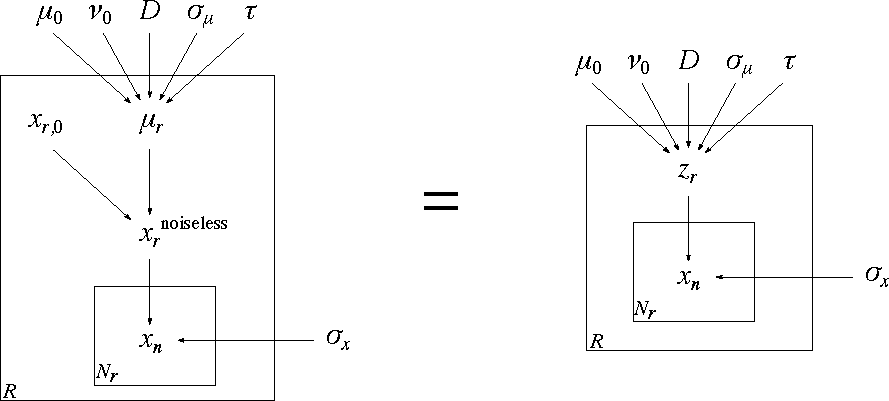
\includegraphics[width=0.7\textwidth]{./figs/graphical_model.pdf}
\end{figure}

To simplify notation and calculations, we package the elements of $x_0, \mu_1, \mu_2$ in a single vector $\tilde z\in \mathds{R}^{3R}$ in an interleaved fashion:
\be
	z_r = (x_{r,0}, \,\mu_{r,1}, \,\mu_{r,2})\quad, \qquad \tilde z = \bigoplus_{r=1}^R z_r
\ee
With this notation, we can eliminate $x_r^\text{noiseless}$ from the graphical representation (because it is deterministic). This is shown on the right side of the figure, and can be written as
\be
	P(x, \tilde z\;|\;\mu_0, \nu_0, D, \sigma_\mu, \tau) = P\Big(\tilde z\;\Big|\; \mu_0, \nu_0, D, \sigma_\mu, \tau\Big) \prod_{r=1}^R P\Big(x^{(r)} \;\Big|\; z_r, \sigma_x\Big)\quad .
\ee

\subsection{Re-ordering $\tilde z$}
To make calculations in the next section easier, we define a re-ordered version of $\tilde z$:
\bel
\label{eq:def_S}
	z =  \left[\bigoplus_{r=1}^R x_{r,0}\right]\oplus \left[\bigoplus_{r=1}^R (\mu_{r,1}, \mu_{r,2})\right] = S \tilde z\quad ,
\eel
where $S = (S_{i,j}\;:\; i,j\in\{0,1,2\ldots R-1\})$ is the permutation matrix expressed with zero-based indexes
\ba
	S_{i,j} = \left\{
	\begin{array}{ll}
		\big[j = 3i\big] &, \quad \text{if}\quad i \leq R-1 \\
		\big[j = i - R + 1 + \lfloor (i-R)/2\rfloor\big] &, \quad \text{if}\quad i \geq R
	\end{array}
	\right.
\ea
where $[\ldots]$ is one if the statement inside if true and false otherwise, and $\lfloor \ldots \rfloor$ indicates the floor function.

We will use the $S$ matrix to convert between the ordering of $\tilde z$ and $z$. As an example, we expand $S\tilde z = z$ for $R=4$  explicitly:
\be
	S\tilde z
	\qquad = \qquad
	\left[
	\begin{array}{ccc|ccc|ccc|ccc}
		1 &   &   &   &   &   &   &   &   &   &   &   \\
		  &   &   & 1 &   &   &   &   &   &   &   &   \\
		  &   &   &   &   &   & 1 &   &   &   &   &   \\
		  &   &   &   &   &   &   &   &   & 1 &   &   \\
		  \hline
		  & 1 &   &   &   &   &   &   &   &   &   &   \\
		  &   & 1 &   &   &   &   &   &   &   &   &   \\
		  &   &   &   & 1 &   &   &   &   &   &   &   \\
		  &   &   &   &   & 1 &   &   &   &   &   &   \\
		  &   &   &   &   &   &   & 1 &   &   &   &   \\
		  &   &   &   &   &   &   &   & 1 &   &   &   \\
		  &   &   &   &   &   &   &   &   &   & 1 &   \\
		  &   &   &   &   &   &   &   &   &   &   & 1
	\end{array}
	\right]
	\quad
	\left[
	\begin{array}{c}
		x_{1,0}   \\
		\mu_{1,1} \\ 
		\mu_{1,2} \\
		\hline
		x_{2,0}   \\
		\mu_{2,1} \\
		\mu_{2,2} \\
		\hline
		x_{3,0}   \\
		\mu_{3,1} \\
		\mu_{3,2} \\
		\hline
		x_{4,0}   \\
		\mu_{4,1} \\
		\mu_{4,2} 
	\end{array}
	\right]
	\quad = \quad
	\left[
	\begin{array}{c}
		x_{1,0}   \\
		x_{2,0}   \\
		x_{3,0}   \\
		x_{4,0}   \\
		\hline
		\mu_{1,1} \\ 
		\mu_{1,2} \\
		\mu_{2,1} \\
		\mu_{2,2} \\
		\mu_{3,1} \\
		\mu_{3,2} \\
		\mu_{4,1} \\
		\mu_{4,2} 
	\end{array}
	\right]
	\qquad = \qquad
	z
\ee



